\section{Variable Name Generation Model}
\label{sec:name-gen}

\begin{figure*}[ht]
	\begin{center}
	  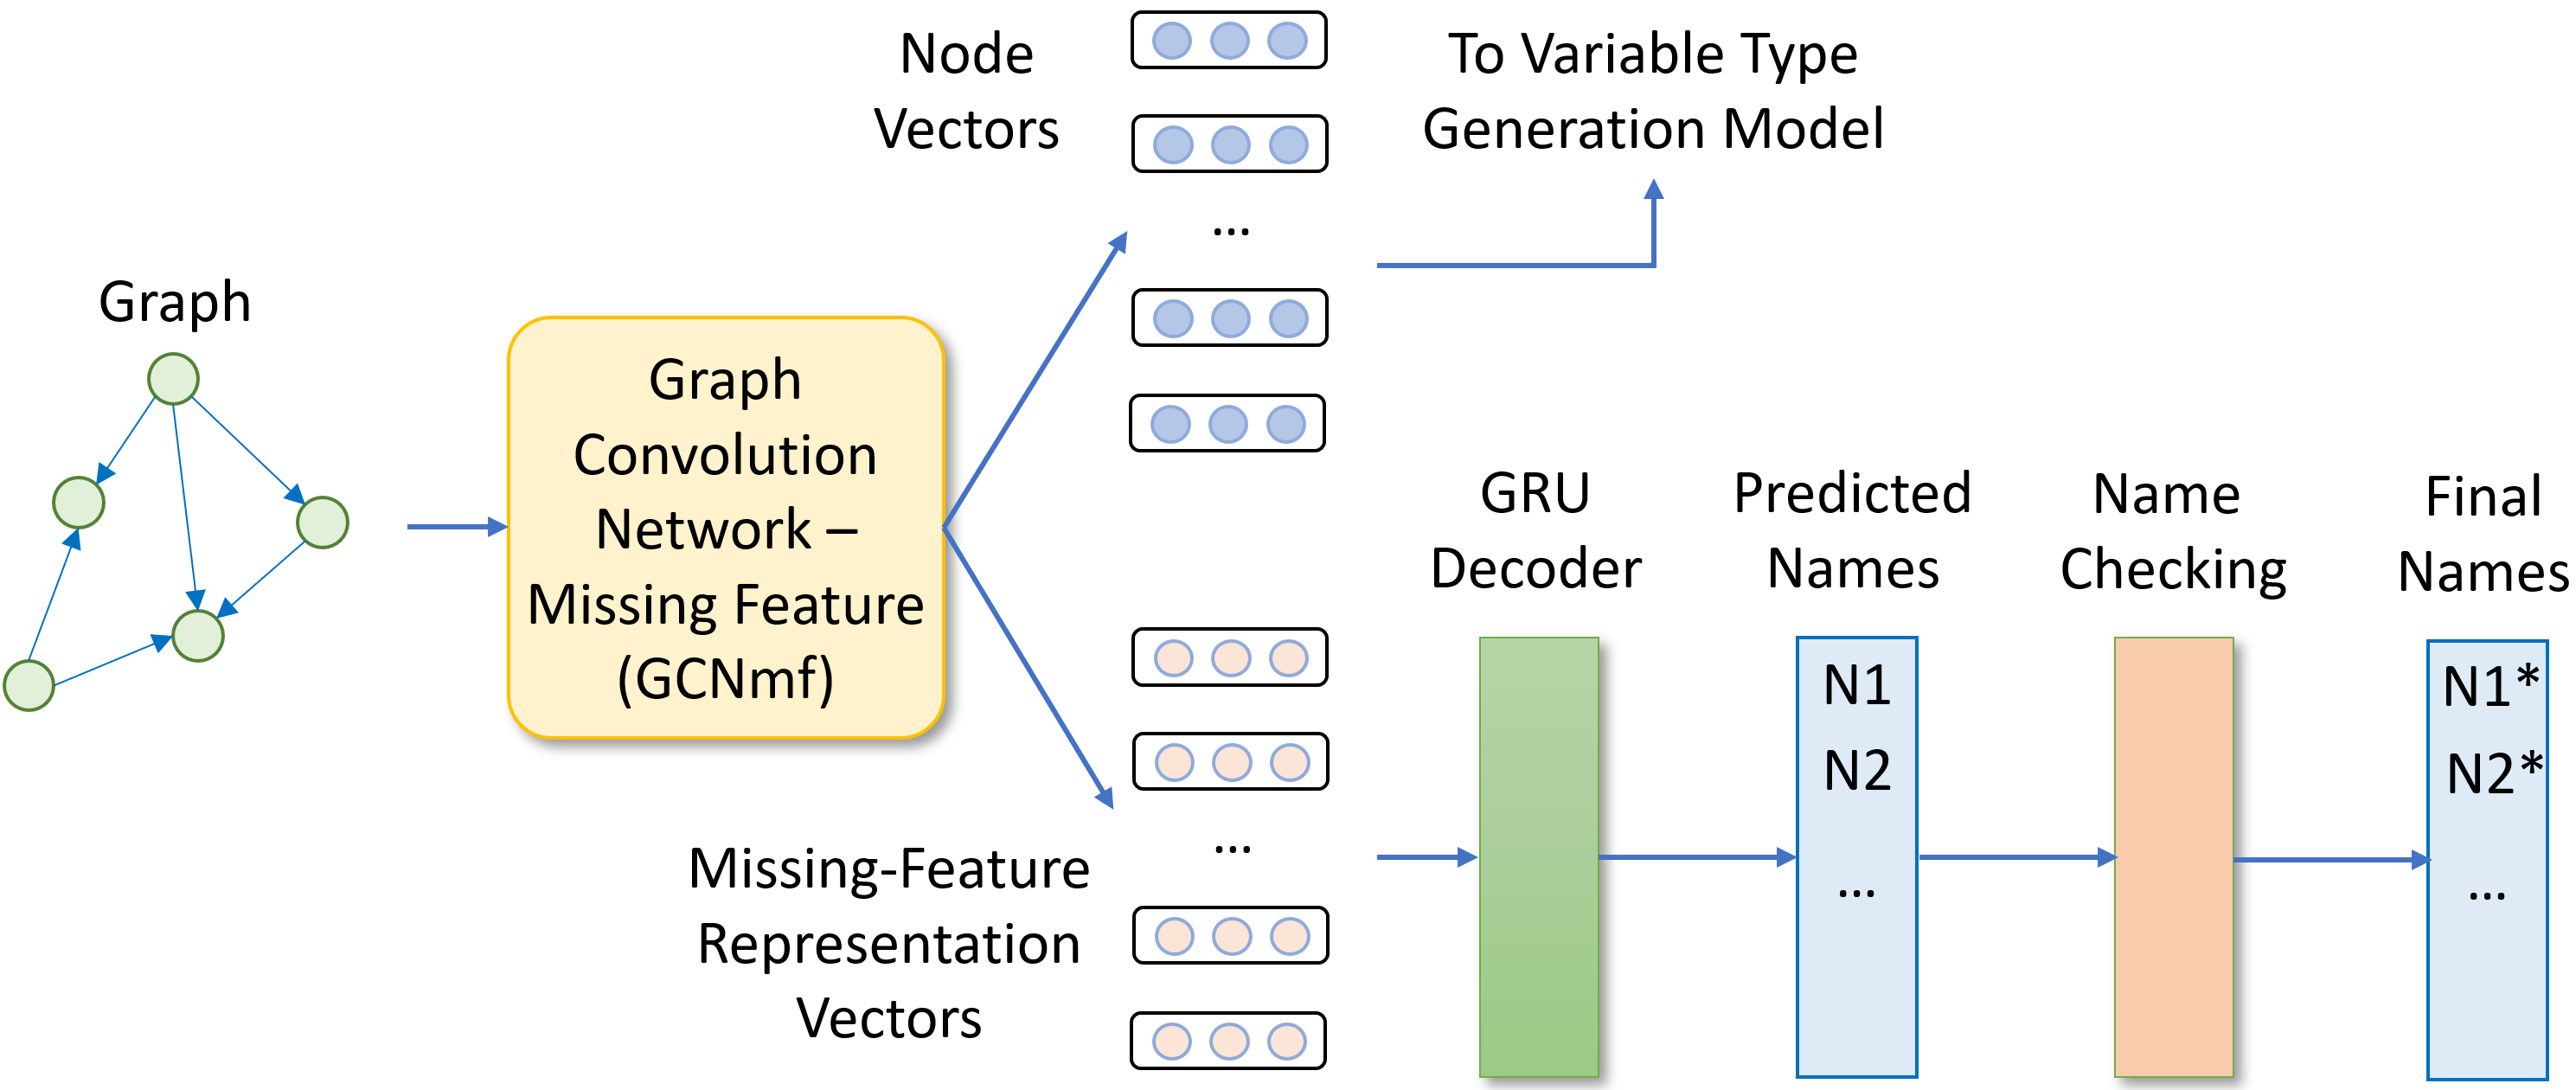
\includegraphics[width=4.7in]{figures/name-gen-model}
          \vspace{-6pt}
		\caption{Variables Name Generation Model (VNG)}
		\label{fig:name-gen}
	\end{center}
\end{figure*}

This section presents the Variable Name Generation Model (VNG).  The
input is the minified code with all the original variables' names and
types during training, and without the names during
prediction. Similar to VTG model, the combined graph $G$ is processed
in which the names in the code sequence of each node $n$ is tokenzed
and an embedding model is applied to build the vector for $n$
considering each sequence of sub-tokens for $n$ as a sentence.

Next, for training, we process the graph $G$ with the node vectors as
follows. For the node $n$ that represents a variable with minified
name, we perform masking the node feature with a special mask token
for the variable name and consider it as a missing feature. Unlike the
VTG model, the VNG model leverages an advanced neural network called
Graph Convolution Network - Missing Features (GCNmf)~\cite{GCNmf}.
The actual names are used as the ground truth labels to train the
GCNmf model. The key characteristic of GCNmf is its ability to deal
with incomplete and missing features in a GCN. It represents the
missing data by Gaussian Mixture Model (GMM) and calculates the
expected activation of neurons in the first hidden layer of GCN, while
keeping the other GCN layers unchanged. The GMM parameters and GCNmf
weight parameters are learned within the same architecture, enabling
the learning of missing features. The GCNmf model is trained with the
masks for the minified variable names. For prediction, applying on the
minified code (without names), the GCMmf model outputs the vectors not
only for the nodes in the graph $G$ but also the vectors for the
missing features.

The vectors representing the missing features, i.e., the missing
variables' names in the input graph $G$ are used next to be fed into a
GRU decoder as in the VTG model (Figure~\ref{fig:name-gen}). The
decoder accepts the vectors for missing names as input and generates
the names for the variable nodes (During training, the name labels are
known and used). Finally, we apply the semantic checkers to make sure
that the variables' names are valid in the scope and that the same
variable is assigned with a consistent name.


%1> Similar to step 2, we use GloVe to learn the representation vector.

%2> For the node that represent the variable with minified name, we mask the node feature and regard it as the missing feature.

%3> Put the graph with missing feature for some nodes into the $GCN_{mf}$ as input. 

%4> The $GCN_{mf}$ can output the predicted missing node feature representation vector $V_{rm}$ and the node representation vector $V'_r$. The node representation vector $V'_r$ will be used in step 2.

%5> Use $V_{rm}$ as the input of a GRU (RNN) decoder, and the decoder generate the names for the variables with the minified name.

%6> When doing generation, we apply basic checking to make sure the same variable has only one consistent name.


%Multi-task learning

%We use the uncertainty weighted multi-task loss as the multitask learning loss function and use the maximum of the top-1 accuracy score from two tasks as the training target.
